\chapter{Evaluation}

( DONT MIND THIS CHAPTER AS MOSTLY SOFTWARE FOR THIS PART IS CURRENTLY WRITTEN AND CONTAINS ONLY THE BARE ESSENTAIL THOUGHS)

With the eventual growth of the Lightning Network a fee market for channel liquidity will emerge. How routing nodes 

\section{Lightning network as a graph}

The Lightning Network may be modeled as a directional Graph $G$ with vertices representing nodes and edges representing channels. As each channel may have different fees and liquidity it's useful to represent each channel with two edges. 



\section{Fee as a competitive equilibrium}

The

The conventional long run demand and supply curve apply to the fee market.

If a demand is running DD' and Supply SS' and

Suppose the average fee price is set at $F_{1}$ with demand $F_{1}D_{1}$ and supply $F_{1}S_{1}$.

\begin{figure}[!htb]
	\hspace*{-0.7cm} 
	\centering
	\includegraphics[width=11cm]{images/equilibrium_sized.png}
	\caption{ 
		}
		\label{fig:equilibrium}
		\hspace*{2mm} 	
\end{figure}

The cost of procuring a shortest path between s and d might be unequal for two different routing nodes dependent on already existing paths and set policies.

\section{Optimal fee pricing}

To determine the fee price, one could intuitively imagine that and increased fee price would yield higher fees but for less pairs as other paths may become shorter. It would be useful to have a more rigid definition of how many shortest paths pass through a vertex. Freeman did so with the introduction of a measurement named \textit{Betweenness Centrality}\cite{freeman:betweenness:centrality} and defined it as

\[ g(v) = \sum_{s \neq v \neq d}\frac{\sigma_{sd}(v)}{\sigma_{sd}} \]

Where $\sigma_{sd}$ are all shortest paths from s to d and v is vertex. As the fee is determined on an edge basis the definition is altered to regard edges instead of vertices. 

It is possible to determine the optimal fee for an edge if some assumption, of the probability of all pairs transacting and the probability of the size of the transactions, are made. If a uniform probability over all pairs and that the shortest paths are used are assumed the optimal price is given by

\[ x_{opt} \textrm{ is the optimal price } iff \]

\[ f: X \to \mathbb{Z} \textrm{ and } (\forall x \subseteq X)f(x_{opt}) \geqslant f(x) \textrm{ where }\]

\[ f(x) = x\sum_{s \neq e \neq d}\frac{\sigma_{sd}(e(x))}{\sigma_{sd}} \]

Where $\sigma_{sd}(e(x))$ is 1 if one shortest path exists over edge e when the edge weight is x or 0 if no shortest path exists.

The function $f(x)$ behaves as seen in figure \ref{fig:fee_curve} for generated graph. 

\begin{figure}[!htb]

	\centering
	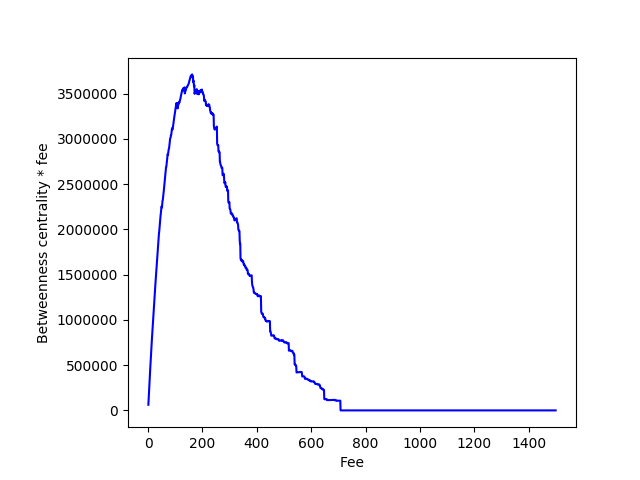
\includegraphics[width=8cm]{images/fee_curve.png}
	\caption{ Shows the betweenness centrality * fee / fee for an edge in a generated graph with 1000 vertices, 5000 edges, uniform weight distribution over 1-1500 and random attachment policy. It holds intuitively as for low fees, many shortest paths passes but procure small overall profits as the fee is small. The profits increases with the increase in fees until a point where the decrease in paths overtakes the increase in fees.
	}
	\label{fig:fee_curve}

\end{figure}

\newpage

Freeman also defined a centrality measurement for whole graphs, it utilizes the betweenness centrality of every vertex and is thus brutal to calculate in practice for larger graphs. 

Efficient algorithms for edge betweenness centrality have been developed\cite{brandes:betweenness:centrality:algorithm}. Although it is possible to run such an algorithm for each potential fee price to find the optima it would be very slow.
Instead the optimal fee price an for outgoing channel $e$, still holding the assumptions as before, may be calculated by following steps.

\begin{enumerate}
	\item Calculate the shortest path from all-to-all vertices without going through $e$ with either Floyd-Warshall or Johnson\cite{johnson:shortest:path:sparse:network} obtaining table A.
	\item Calculate shortest path from the source of $e$, $V$-to-all explicitly going through $e$ with Dijkstra obtaining table D where $e$ weight set to 0.
	\item Retrieve the difference for all pairs between the all-to-all distance with the all-to-$V$-to-all distance, A[s][d] - (A[s][V] + D[d]). Throw away the negative values and produce a cumulative summation over the differences in a table H.
	\item Select $x_{opt}$ such that \[ \forall x (x H(x)) \leq x_{opt} H(x_{opt}) \]
%	 producing a cumulative summation over the difference.\\
%	For all pairs s, d:\\
%		If $A[s][d] > A[s][i] + S[d]$ \\
%		then $D[A[s][d] - (A[s][i] + S[d])] += 1$.\\
	
	
		%\[ M_i := \sum_{s \neq d}^{i} A[s][d] > A[s][i] + D[d]  \]
%	\[ \sum_{s \neq d} 
%	\begin{cases}
%		A[s][d] - A[s][i] + D[d],& \text{if } A[s][d] > A[s][i] + D[d]\\
%		0,              & \text{otherwise}
%	\end{cases} \]


\end{enumerate} 

Whenever Floyd-Warshall or Johnson should be used depends on the sparseness of G as Floyd-Warshall have a time complexity of

\[ O(V^3) \]

only dependent on vertices whereas Johnson

\[ O(V^2 log(V) + VE ) \]

depends on both edges and vertices. 

\section{Topology}

Network topology

\[ P(k) \propto k^{-\gamma} \]

\[ p_i = \dfrac{k_i}{\sum_{j}^{}k_j}  \]


Lightning network consists of nodes playing game

Non routing nodes, cheap as possible and possible as private as possible(?) 

Barabási–Albert model

Does it become scale free

does any channel opening algorithm perform better than another and essentially force the network into a scale free hub-spoke network instead of a mesh network?
 



\newpage
\onecolumn

\begin{figure}[!htb]
	\hspace*{-0.7cm} 
	\centering
	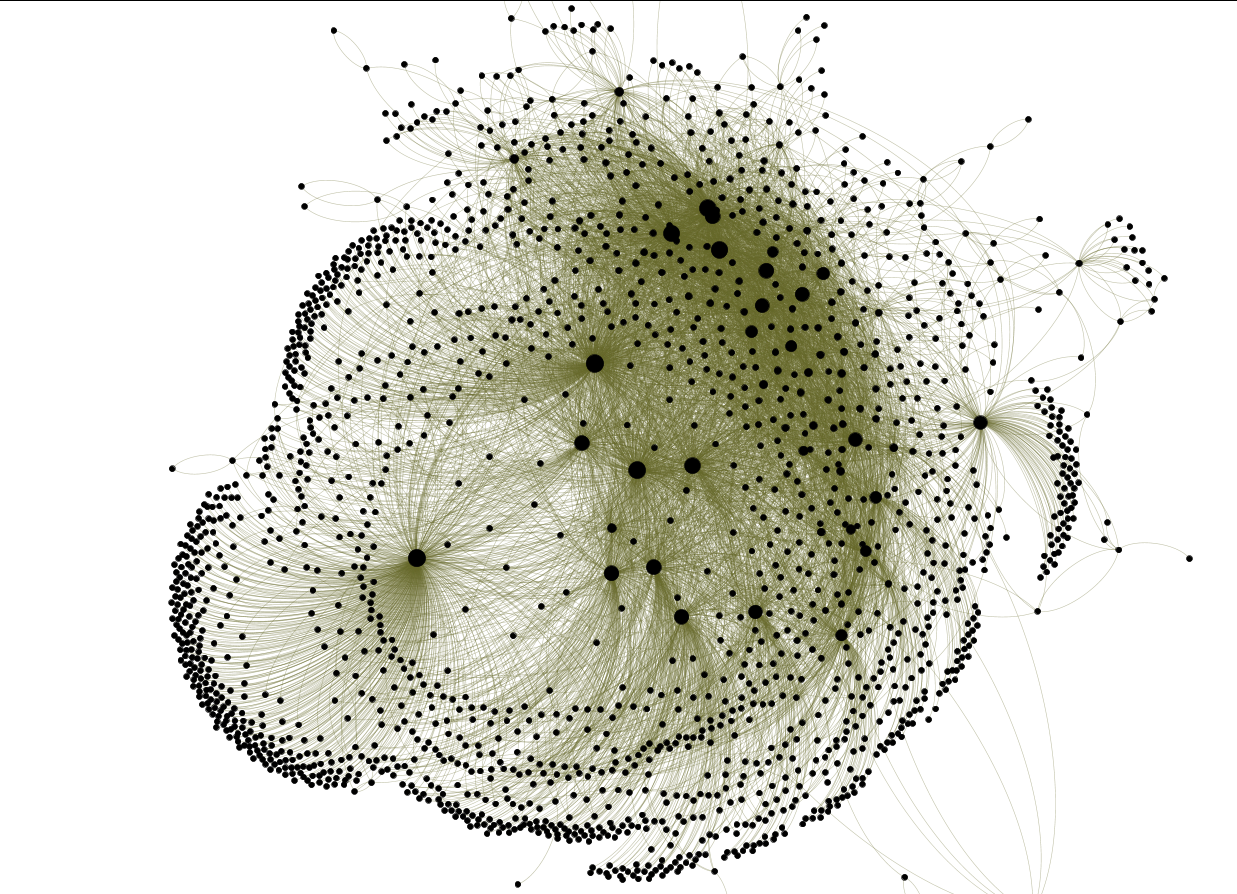
\includegraphics[width=12cm]{graphs/testnet_force.png}
	\vspace*{-0.4cm} 
	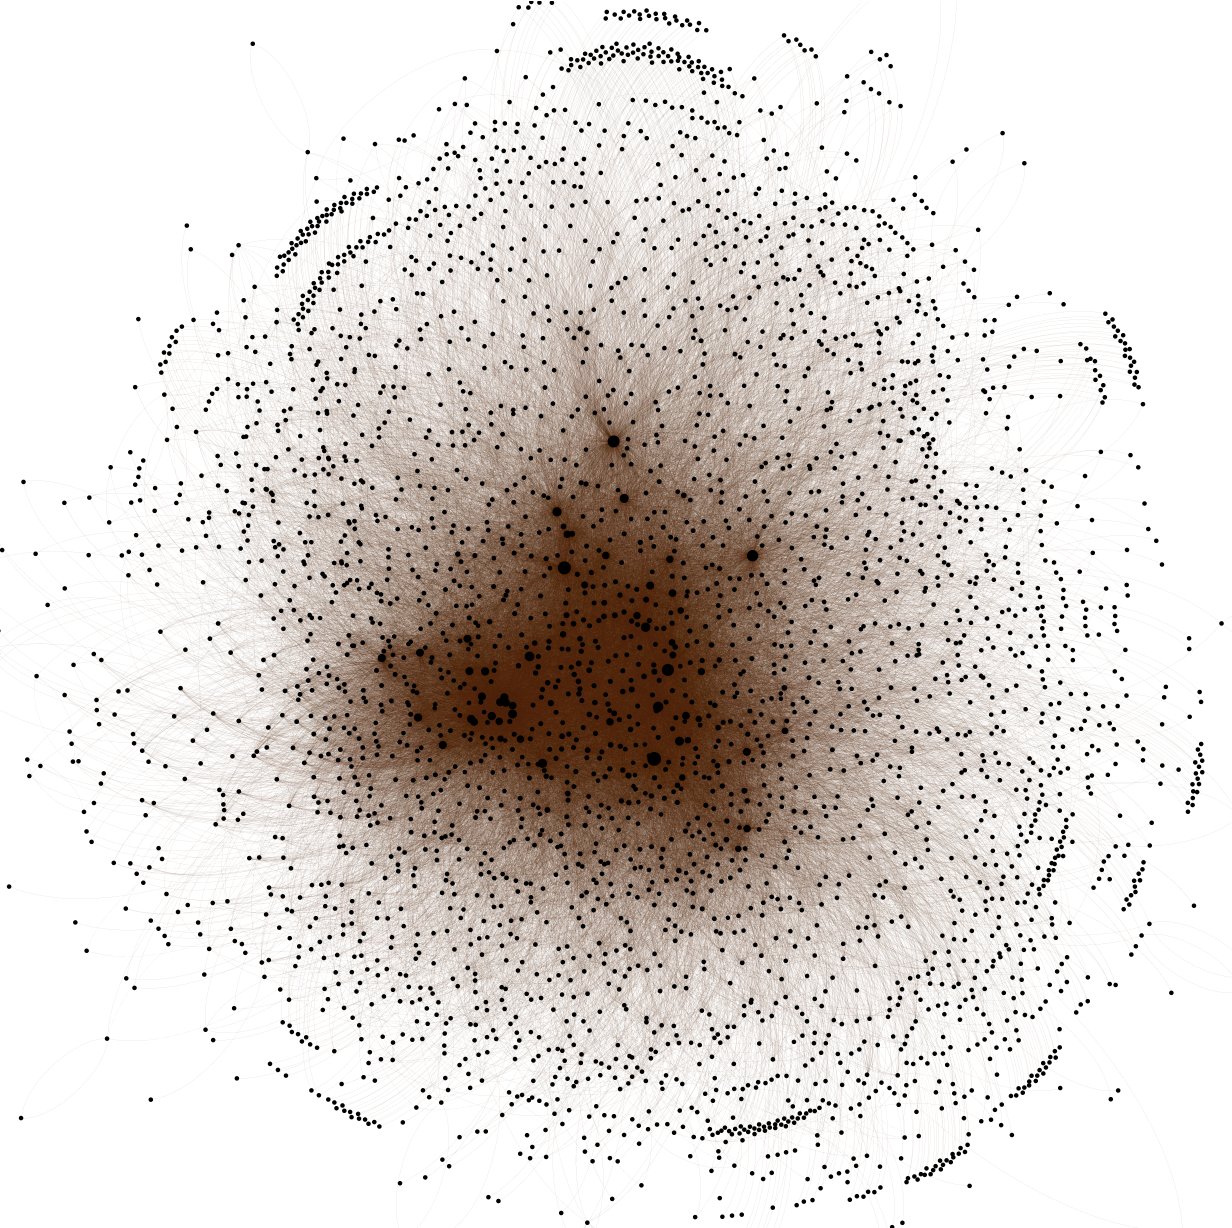
\includegraphics[width=13.6cm]{graphs/mainnet_force3.png}
	\caption{\textit{
		Shows testnet above and mainnet below as of 2019-02-25. Node size corresponds to degree, larger degrees to larger size. Positioning is a mix between Force Atlas and Fruchterman Raingold. Network data retrieved by running a c-lightning node and visualized with Gephi\cite{repository:gephi}.}}
	\label{fig:equilibrium}
	\hspace*{2mm} 	
\end{figure}
\newpage
\twocolumn


% THE ADJUSTABLE SCALE FREE  http://www.uvm.edu/pdodds/files/papers/others/2002/holme2002a.pdf



% https://webusers.imj-prg.fr/~ricardo.perez-marco/publications/articles/antrouting3.pdf

% https://bitfury.com/content/downloads/whitepaper_flare_an_approach_to_routing_in_lightning_network_7_7_2016.pdf

% https://en.wikipedia.org/wiki/Betweenness_centrality